

\section{プログラムの説明}
本課題では,検索した都市の天気情報を取得するWebアプリケーションを作成した(図\ref{fig:full}).以下では作成したプログラムを本アプリと呼称する.

本アプリは大きく3つのパーツに分かれており,ページ画面の上から,検索フォーム,天気情報の詳細表示,日付ごとの天気情報リストとなっている.
本アプリでは,これらのパーツのみで内部的な画面遷移を行なっており,外部ページへのリンクは行っていない.

本アプリの機能としては以下のものがある.
\begin{itemize}
\item 検索した都市の天気情報の取得.
\item 特定の日付の詳細な天気情報の表示.
\item 検索日から6日間の天気情報一覧リストの表示.
\end{itemize}

例えば,検索フォームに「福岡」と入力すると,福岡市の今日の詳細な天気情報が表示され,その下には今日から5日後までの天気情報一覧リストが表示される.
一覧リストから日付を適当に選択すると,その日付の天気予報の情報が表示される.

本アプリの作成にあたって,フレイムワークとして\href{https://jp.vuejs.org}{Vue.js},天気情報取得のAPIとして\href{https://openweathermap.org}{OpenWetherMap}を用いた.
%本アプリの作成にあたって,フレイムワークとしてVue.js,天気情報取得のAPIとしてOpenWetherMapを用いた.

\begin{figure}[htbp]
\centering
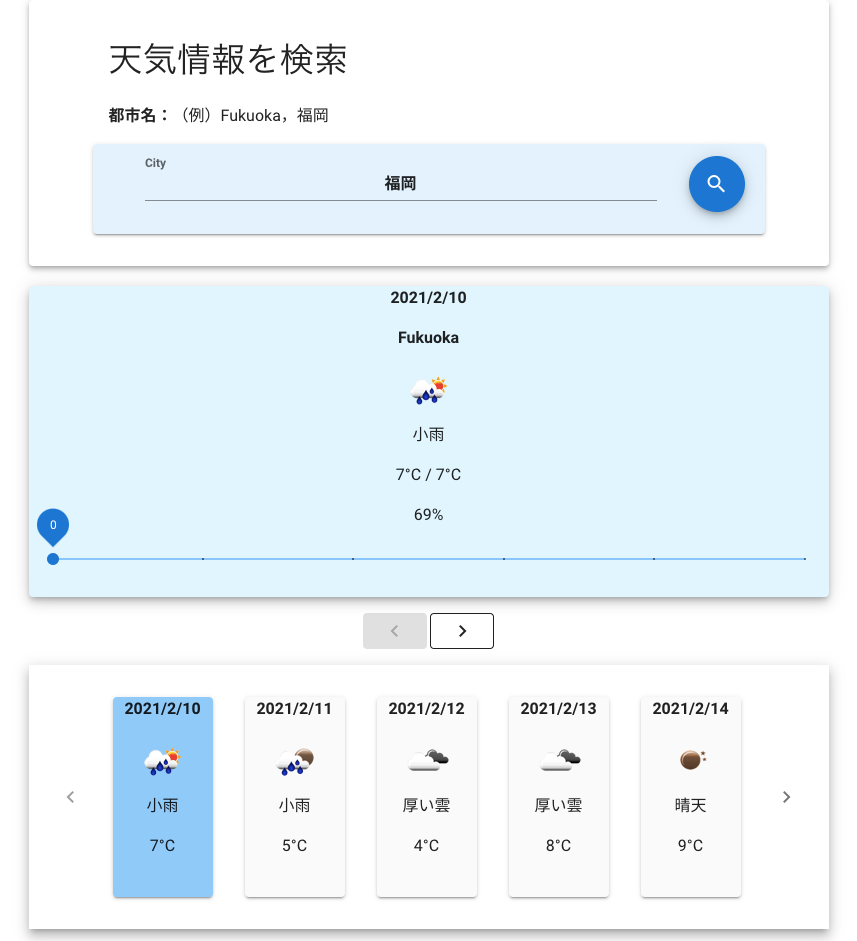
\includegraphics[width=15cm]{full1.png}
\caption{Webページの全体像}
\label{fig:full}
\end{figure}


\section{工夫した点}

\subsection{アプリの初期状態}
本アプリを開くと,まず検索フォーム(図\ref{fig:top})のみの画面が表示される.このときユーザが行える操作は検索フォームに都市名を入力することと,検索ボタンをクリックすることだけである.
これは,情報を少なくして限定することによって,初めて本アプリを使うユーザでも混乱せずに,何をすれば良いのかを理解しやすくするためである.都市名を入力し検索ボタンをクリックして初めて,検索フォームの下に都市の天気情報が表示されるようになる.

\subsection{ホバーエフェクト}
本アプリのパーツや構成要素はマテリアルデザインを参考にし,パーツはそれぞれカード形式を採用した(図\ref{fig:full}).これは各パーツをカードで分別することで,パーツそれぞれの機能を明確にするためである.それぞれのパーツにおいて操作できる部分は,検索フォームの入力欄と検索ボタン,天気情報でのスライドバーと進む・戻るボタン,日付リストのそれぞれのアイテムである.これらはマウスによって操作することができるが,操作可能なことを明示するために,これらの要素にホバーエフェクトを加えた.ホバーエフェクトは,マウスカーソルを合わせた時にその部分が浮き出て強調表示されるようなエフェクトである.これによってユーザは,どこが操作可能かをマウスを移動させることで直感的に理解することが可能である.

\subsection{スライドバー}
本アプリの天気情報詳細表示のパーツにおいて,スライドバーを導入している(図\ref{fig:main}).このスライドバーの役割は,今表示されている天気情報が今日から何日後のものかを明示するものである.例えば,図\ref{fig:main}のようにスライドバーの値が2となっているときは,今表示されている天気情報が今日から2日後のものであると示しており,図\ref{fig:full}のように値が0となっているときは,今日の天気情報が表示されていることを表している.そのため,日付一覧リストで選択されている日付に対応して,スライドバーの値が変動する仕組みである.

スライドバーのもう一つの役割は,日付の容易な操作である.本アプリで日付を変更する方法として,日付一覧リストからアイテムをクリックしてその日付を直接選択することと,進む・戻るボタンから1日前・1日後の日付を選択することの2つに加えて,スライドバーを直接スライドさせることでも日付を変更することが可能である.スライドバー以外の2つの方法の方が直感的な操作が可能であるが,これらはそれぞれ,日付リストに表示されている6日のうちから選択,または1日ずつ変更することでしか一度に日付の操作ができない.取得できる天気情報の日数が増えたとき,これらの操作方法よりもスライドバーを利用した一気に日付を変更する方法の方が便利である.

\subsection{アイコン}
本アプリでは,できるだけ文字による説明を行わず,様々な情報をアイコンで表示することで,ユーザによる直感的な操作の理解を狙った.例えば,検索ボタン,日付を変更する進む・戻るボタン,日付ごとの天気の簡易情報はそれぞれアイコンによって表示している.このように文字による説明を最小限にしたことによって,本当に重要な情報である検索フォームにおける都市名の説明や,詳細な天気情報といった文字情報にユーザが目を向けやすくすることも目的としている.


\begin{figure}[htbp]
\centering
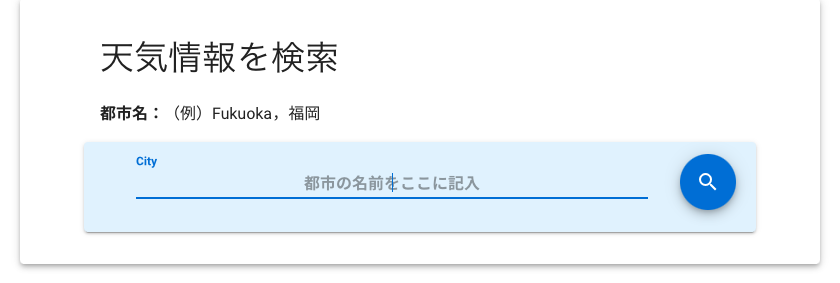
\includegraphics[width=15cm]{top1.png}
\caption{天気情報の検索フォーム}
\label{fig:top}
\end{figure}

\begin{figure}[htbp]
\centering
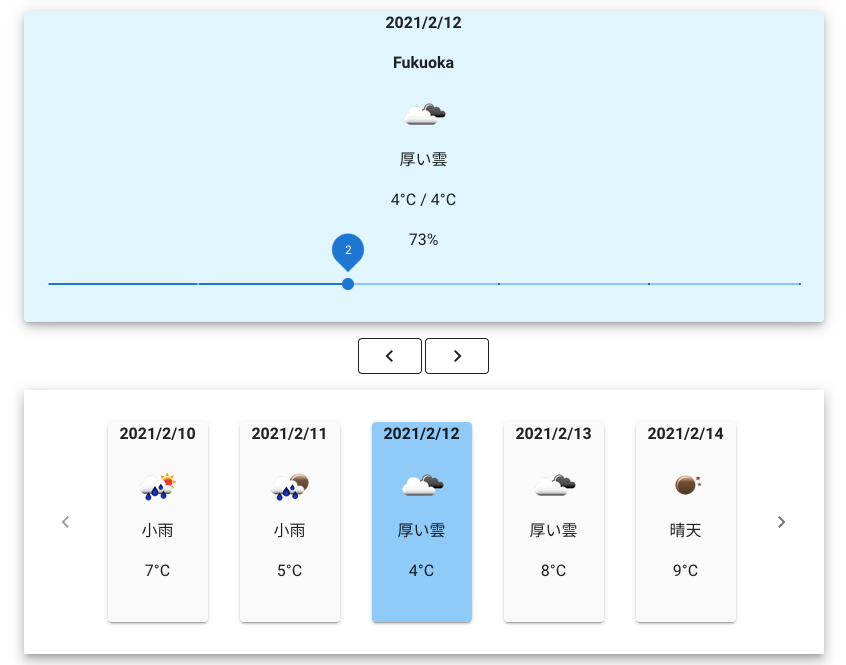
\includegraphics[width=15cm]{main2.png}
\caption{日付リストとスライドバー}
\label{fig:main}
\end{figure}


\section{改善案}

\subsection{アプリの初期状態}
本アプリの初期状態で検索フォームのみを表示し情報を限定したことで,アプリ操作の単純化を図った.しかし,図\ref{fig:top}のように検索フォームがWebページの上部に表示されるだけであり,その下は全くの空白となっている.これはユーザインタフェースとしてバランスが悪く,ユーザに不必要な違和感を与える可能性がある.その改善案として,まず本アプリの簡潔な説明と検索フォームをまとめてフルページで表示し,都市を検索すると天気情報が表示される新しいフルページに画面遷移するものが考えられる.このようにすれば,初期状態の簡潔さを失うことなく,インタフェースとしてのバランス悪さを回避することが期待できる.

\subsection{日付の変更}
本アプリでは天気情報における日付の変更方法として,スライドバーを用いた.スライドバーによって日付の補助的な情報の付与,および取得できる日数に依存しない簡易な日付変更を可能にした.しかし,本来スライドバーは対象となる値の入力や調整に使われるユーザインターフェイスであり,本アプリでの利用方法は斬新なものと言えるが,本来の使い方からずれていることからユーザの混乱を招く恐れがある.その改善案として,スライドバーの代わりにカレンダーによる日付の変更を行うものが考えられる.日付一覧リストもスライダー形式を用いたものではなく,カレンダーによる一覧表示にし,カレンダー内の日にちを選ぶことで日付の変更を可能にすれば,直感的な操作および取得できる日数に依存しない簡易な日付変更を両立できることが期待できる.

